\section{JoystickControl}\insertloftspace
\setcounter{figure}{0}\setcounter{table}{0}

\subsection{Principle}

\hspace{\parindent} The initial request of our customer was a remote controlled arm. This was the easiest and fastest solution to implement. Mr. Kedziora also wanted to avoid using artificial intelligence in order not to lengthen the prototype manufacturing time.

\bigbreak
In this configuration, a camera, fixed on the arm at the level of the hand, allows the user to have a video return. An Xbox controller in our case is used to control the arm. The commands sent by the user are done in the camera's frame.

\begin{figure}[ht]
    \centering
    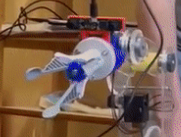
\includegraphics[width=0.8\textwidth]{images/Section06/camera.png}
    \caption{Camera position}
    \label{fig:mesh16}
\end{figure}
\FloatBarrier

\begin{figure}[ht]
    \centering
    \includegraphics[width=0.8\textwidth]{images/Section06/camera\_view.png}
    \caption{Camera view}
    \label{fig:mesh17}
\end{figure}
\FloatBarrier

\bigbreak
As explained in the previous section, the inverse kinematics calculates the necessary angles for a given position in the base frame \{s\}. However, it seemed more natural to us to make the user work in the camera reference frame \{c\} and then to change the reference frame. For this, we reused the modern robotics library. In the same way that we can calculate the transformation matrix between the base and the end effector from the position of the links, we can calculate the one between the base and the camera. 
\begin{center}
    $T_{sc} =\displaystyle \prod_{n=1}^4e^{[S_i]\theta_i}M_c$
\end{center}

\bigbreak
Then the relation between the position in the reference frame and the position in the reference frame is the following:
\begin{center}
    $p_s = T_{sc}p_c$
\end{center}

\bigbreak
Attention, $T_sc$ being a 4x4 matrix, $p_s$ and $p_c$ are homogeneous positions:$p = [p\hspace{0.2cm}1]$. At each command sent by the user, we retrieve the position of each of the links and then we apply the following code that puts into practice the previous equations. We obtain the position in the base frame.

\bigbreak
\begin{minted}[linenos=true,bgcolor=LightYellow]{Python}
    # import kinematics parameters
    from parameters import * 
    import modern_robotics as mr
    # receive angles and desired position from ros 
    thetalist = get_angles()
    p_c = get_position()
    p_c = np.array([p_c 1])
    # get transformation matrix and change the position
    t = mr.FKinSpace(m_c,screw_list,thetalist)
    p_s = np.dot(t,p_c)
    p_s = p[:3]
\end{minted}

\bigbreak
The control of the three axes is done with the two joysticks on the joystick. The left joystick allows to move according to the plane (x,y) of the camera and the joystick manages the depth. Some features listed below have also been added on the buttons to facilitate the work of the user and the proper functioning of the arm.
\begin{itemize}[noitemsep]
    \item authorize the movement: button A
    \item prohibit the movement: button B
    \item return to zero position : button X
    \item return to deposit position : button Y
\end{itemize}

\begin{figure}[ht]
    \centering
    \includegraphics[width=0.8\textwidth]{images/Section06/xbox\_controller.png}
    \caption{Xbox Controller}
    \label{fig:mesh18}
\end{figure}
\FloatBarrier

\subsection{Open loop}

\subsection{Closed loop}
